\chapter{Finite Impulse Response (FIR) Filter Project}
\glsresetall
\label{chapter:FIR_Project}

\section{Introduction}

In this project, you will do three tasks using \VHLS tool and the Zedboard:
\begin{itemize}
\item Design 11 tap FIR filter
\item Demonstrate the 11 tap filter on the Zedboard
\item Design and optimize 128 tap matched filter. 
\end{itemize}

We provide baseline code for the designs and demo. For the 11 tap FIR filter and demo, you must acquire necessary knowledge from the resources provided with this document. For the matched filter, you must perform necessary optimizations to increase the throughput, decrease the latency, and decrease the area. In your report, you must provide the synthesizable code, describe the optimizations and their architectures, and discuss the impact of each optimization on the throughput, latency, and area.

\section{Preparation}
Before you start, we strongly suggest that you go through these high level synthesis tutorials: Lab 1, Lab 2 and Lab 3 in this document: ug871-vivado-high-level-synthesis-tutorial.pdf. You can find this document in the given Tutorial folder. \note{Fix this. Add this document somewhere and point to it.}

\section{Materials}

\note{Need to add a location for this.}
You can find the following files in project1-fir.zip:
\begin{itemize}
\item \texttt{fir11} folder: 11 tap fir filter
\begin{itemize}
\item \texttt{fir.cpp}: Implements top level function
\item \texttt{fir.h}: Header file
\item \texttt{fir\_test.cpp}: Test bench
\item \texttt{input.dat}: Input chirp signal
\item \texttt{out.gold.dat}: ``Golden'' output. When the testbench (from fir\_test.cpp) is run through the file fir.cpp it should generate this result. If it does not, you did something wrong.
\end{itemize}
\item \texttt{fir128} folder: 128 tap matched filter
\begin{itemize}
\item \texttt{fir.cpp}: Implements top level function
\item \texttt{fir.h}: Header file
\item \texttt{fir\_test.cpp}: Test bench
\item \texttt{input.dat}: Input chirp signal
\item \texttt{out.gold.dat}: ``Golden'' output. When the testbench (from fir\_test.cpp) is run through the file fir.cpp it should generate this result. If it does not, you did something wrong.
\end{itemize}
\item \texttt{Demo} folder: Demo folder for 11 tap filter
\begin{itemize}
\item \texttt{host\_fir.c}: Unfinished host program
\item \texttt{exe\_script.sh}: Execution script
\item \texttt{plot\_script.p}: Plotting script
\item \texttt{input.dat}: Input chirp signal
\end{itemize}
\item Tutorial folder
\begin{itemize}
\item \texttt{ug871-vivado-high-level-synthesis-tutorial.pdf}: Various tutorials for Vivado HLS
\end{itemize}
\end{itemize}

\section{Project Goal}
The first goal of this project is to generate a design from HLS (FIR11) and implement it on the Zedboard.  Also you should start to gain an understanding of different HLS optimizations. For FIR128, you should modify the code to generate at least four additional architectures. Your goal is to create architectures that provide tradeoffs between area and execution time. This will require you to rewrite the code and/or insert pragmas. Your final assignment must contain followings:
\begin{itemize}
\item Design a 11 tap fir filter with HLS. In the rest of this document, we use the term \term{FIR11} to refer this task.
\item Demo for FIR11: In the rest of this document, we use the term \term{Demo} to refer this task. 
\item Design 128 tap fir filter with HLS and optimize it. In the rest of this document, we use the term \term{FIR128} to refer this subtask.
\end{itemize} 

\section{FIR11}

The first step for the project is to get a functionally correct design working for an 11 tap FIR filter. For this, you will need to use the \VHLS tool, and finish the function body of \texttt{void fir()} in the file \texttt{fir.cpp} to implement the filter. You can test the correctness of your code by using the provided testbench. This code does not need to be highly optimized; you will work on creating optimized code later. It just needs to work correctly. This is the code that you will use to program the programmable logic portion of the Zynq chip on the Zedboard. The next step requires that you set up the Zedboard to run Linux on the ARM processor on the Zynq chip, and communicate data back and forth between the ARM processor and your FIR11 core running on the programmable logic. Further details on this are explained in next section.  

\section{Demo}

Following are steps to implement your FIR11 HLS design on the Zedboard. You will provide the input data (chirp signal) from the ARM, and get the output from the Zedboard to the ARM. To do that, you must write a \texttt{host\_fir.c} program. We provided a template of \texttt{host\_fir.c}. Find the comment \texttt{//Add your code here:} and insert your code after that. You also need to write the gnuplot script to plot the output on the GUI. To do this demo you need: a Zedboard, Mouse, Keyboard, Monitor, and USB Hub.

The specific things you must do in this section are:
\begin{itemize}
\item Download two files from: 
\begin{itemize}
\item \url{http://xillybus.com/downloads/xillinux-eval-zedboard-1.3a.zip}
\item \url{http://xillybus.com/downloads/xillinux-1.3.img.gz}
\end{itemize}
\item Read Sections 1 - 4 in the Xillybus tutorial (\url{http://xillybus.com/downloads/doc/xillybus_getting_started_zynq.pdf}). We will use ISE (not Vivado) in this lab since Xillybus does not play well with the current versions of Vivado.  In other words, follow the instructions in Section 3.5.1 in the Xillybus tutorial to generate your bit stream.
\item Read Part I - IV in the Xillybus HLS integration tutorial (\url{http://xillybus.com/tutorials/vivado-hls-c-fpga-howto-1}), integrate your 11-tap FIR HLS design with Xillybus, and
implement your FIR HLS design on the Zedboard. Finish the given host program \texttt{host\_fir.c}. Again, the functions you need are described in this tutorial. Compile your host program (using \texttt{gcc}). Run \texttt{exe\_script.sh} to get this input/output signal graph. The expected output is as shown in Figure \ref{fig:zillybus_fir_demo}.
\end{itemize}

\begin{figure}
\centering
%\includesvg{images/matrix_vector_sequential}
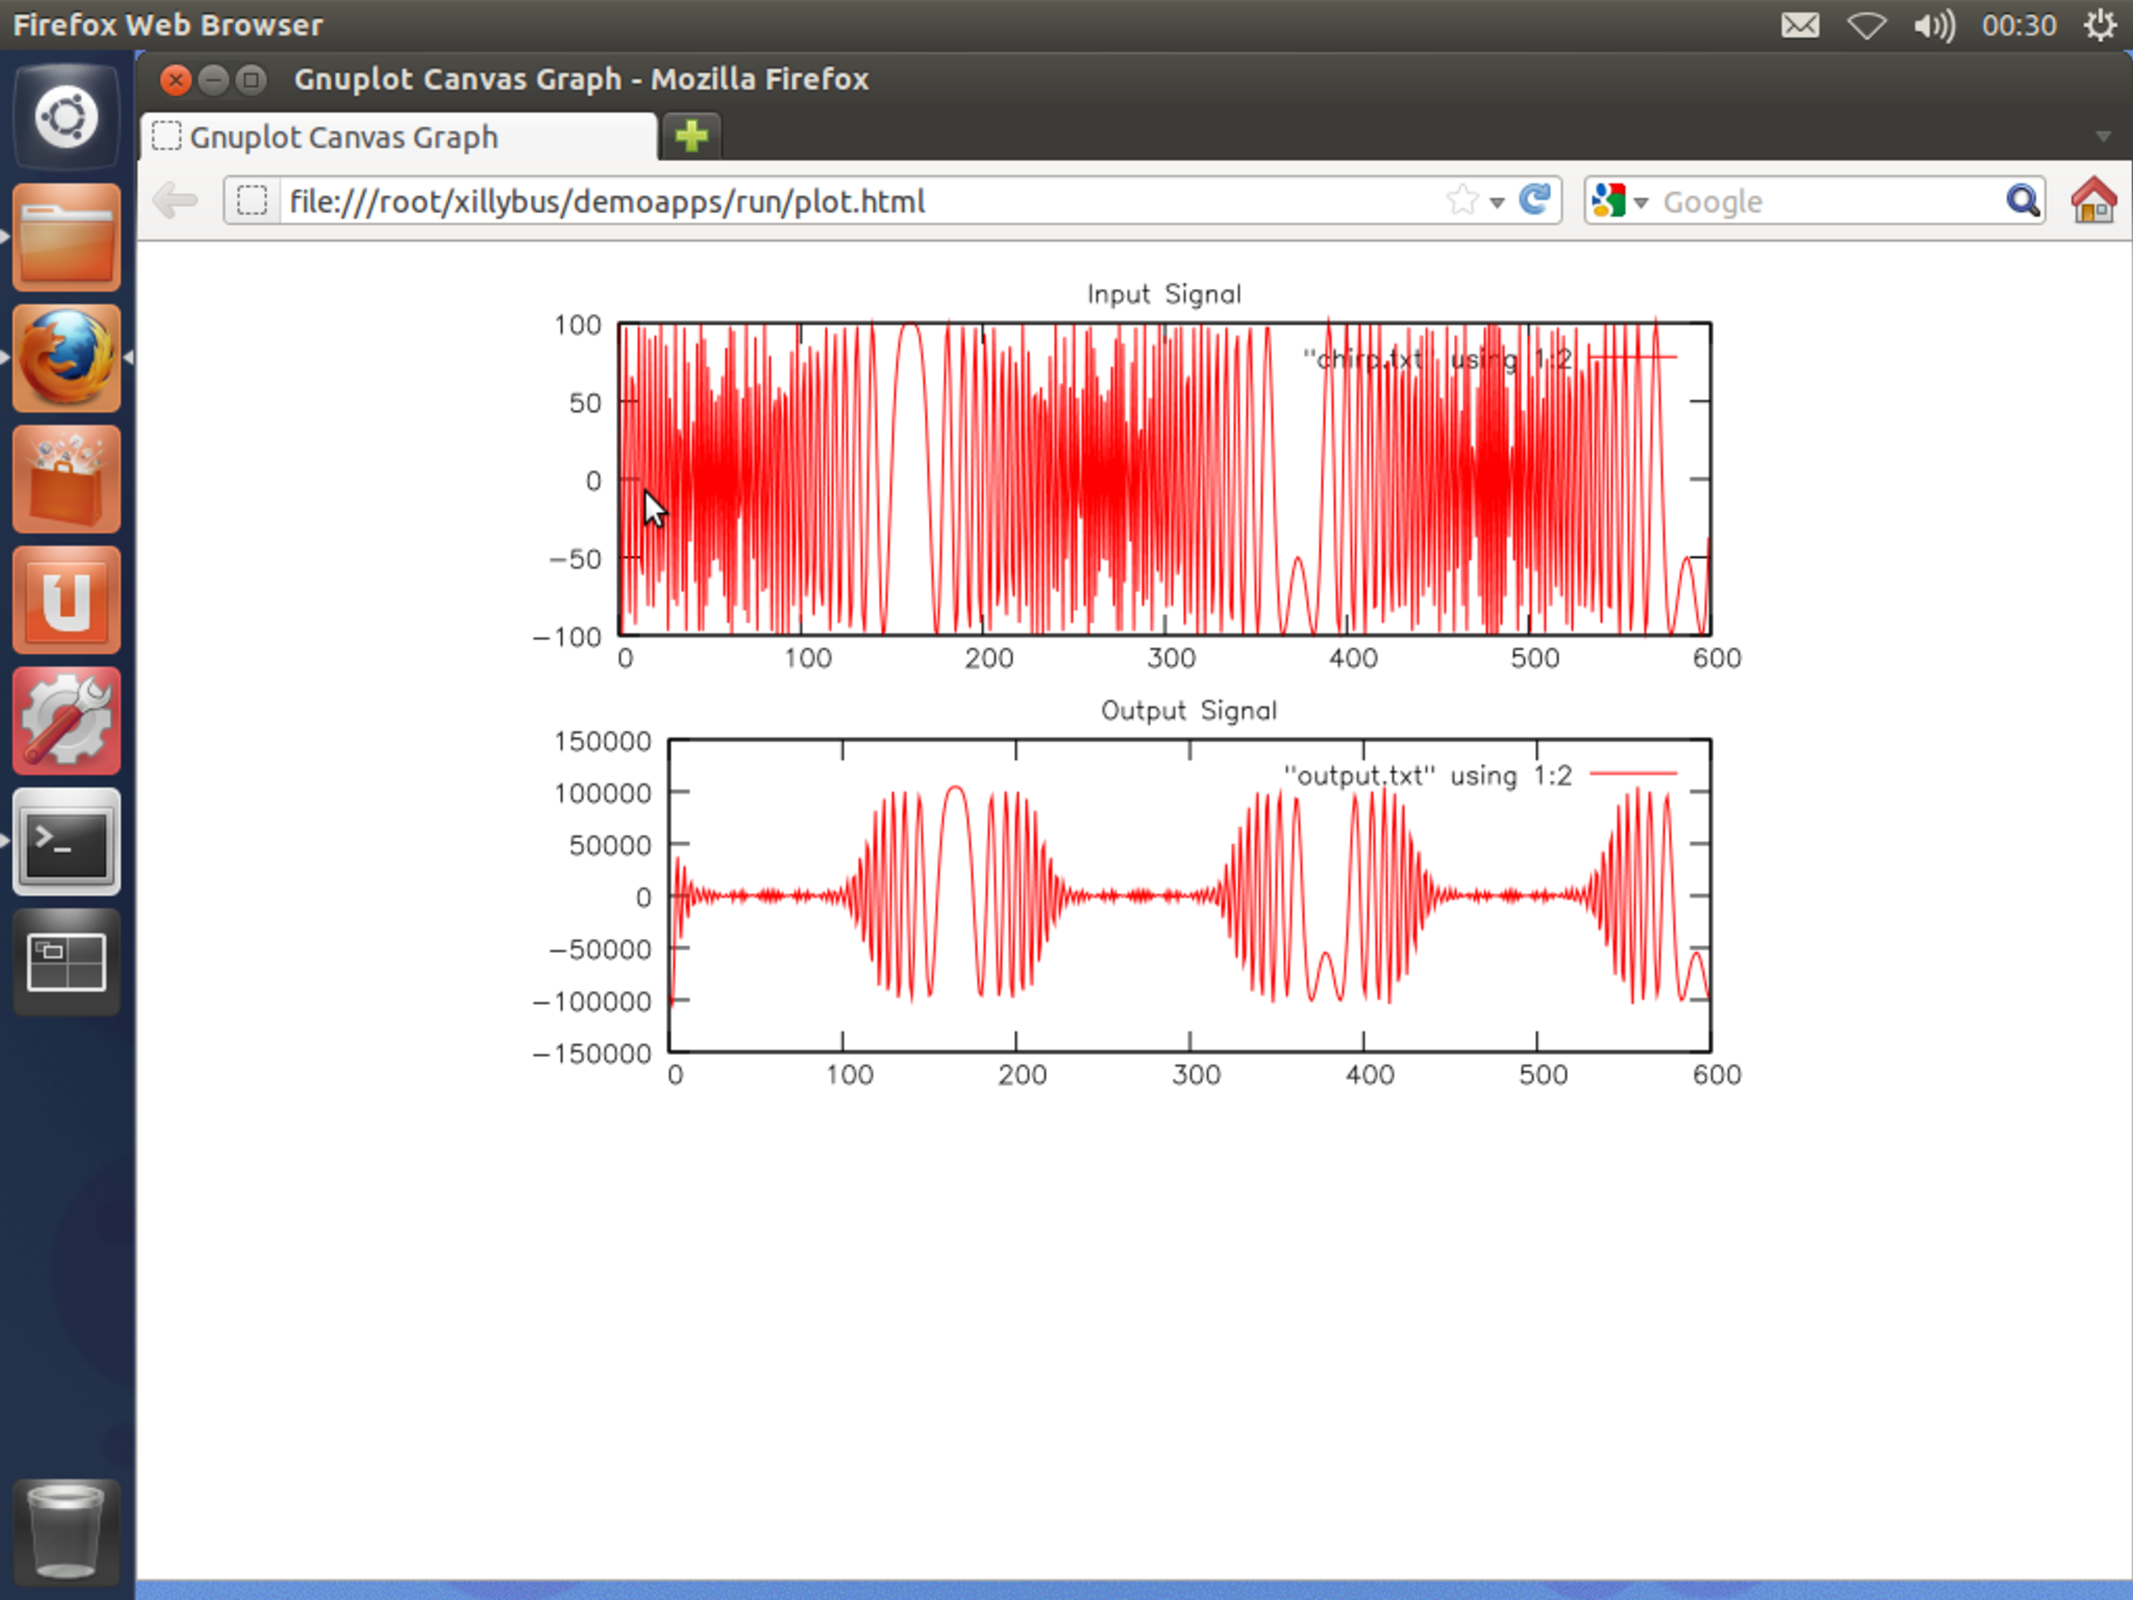
\includegraphics[width=5.5in]{images/zillybus_fir_demo}
\caption{The expected output for the \texttt{FIR11} demo.}\label{fig:zillybus_fir_demo}
\end{figure}

You should submit the graph with your final write up as proof that you got it to work. We also reserve the right to see the demo in person.

\section{FIR128 Optimization Hints}
You must generate at least one architecture that utilizes all of these optimization hints. This architecture does not have to use all of the hints, e.g., you could generate five different architectures where each one performs one of these optimizations. You are free to use any additional optimizations. The only restriction is that your resulting code is correct, i.e., it matches the golden output.
Some possibilities for optimization include:
\begin{itemize}
\item \textbf{Variable Bitwidths:} The bitwidth of the variables provides a tradeoff between precision, area, and performance. It is possible to specify the exact size of each variable to the tools. Make sure that you do not affect the results, i.e., the output still matches the golden output.
\item \textbf{Removing Conditional Statements:} If/else statements and other conditionals limit the possible parallelism and create additional area. If the code can be rewritten to remove them, it typically makes the resulting architecture smaller and faster.
\item \textbf{Pipelining:} This increases the throughput at the cost of adding area (registers). The area and performance can be varied by changing the initiation interval (II).
\item \textbf{Loop Fission:} Dividing the loop into two or more separate loops may allow for each of those loops to be executed in parallel. This will increase the performance and the area.
\item \textbf{Memory Partitioning:} The storage of the arrays in memory plays an important role in area and performance. On one hand, you could put an array entirely in one memory. And this memory can have a different number of ports (e.g., one or two ports for FPGA block RAM). Or you can divide the array into two or more memories to increase the number of ports. Or you could instantiate each of the variables as its own register, which allows simultaneous access to all of the variables at every clock cycle, but has high area costs. 
\end{itemize}

For your designs, you should report performance and area results. Figure \ref{fig:fir_area_results} and Figure \ref{fig:fir_performance_results} provide an example of how to plot the area and performance results. Figure \ref{fig:fir_area_results} plots the number of LUTs, FFs, DSP, and BRAMs used for 8 different designs. Figure \ref{fig:fir_performance_results} shows the performance in terms of number of FIR outputs/second for these 8 designs.  We describe how we calculate the throughput below. Your graphs do not necessarily have to look exactly like these. These are provided as examples. There are many other ways to present the results. However, it is important to make sure to present the results in the most coherent and organized manner as possible.

\begin{figure}
\centering
%\includesvg{images/matrix_vector_sequential}
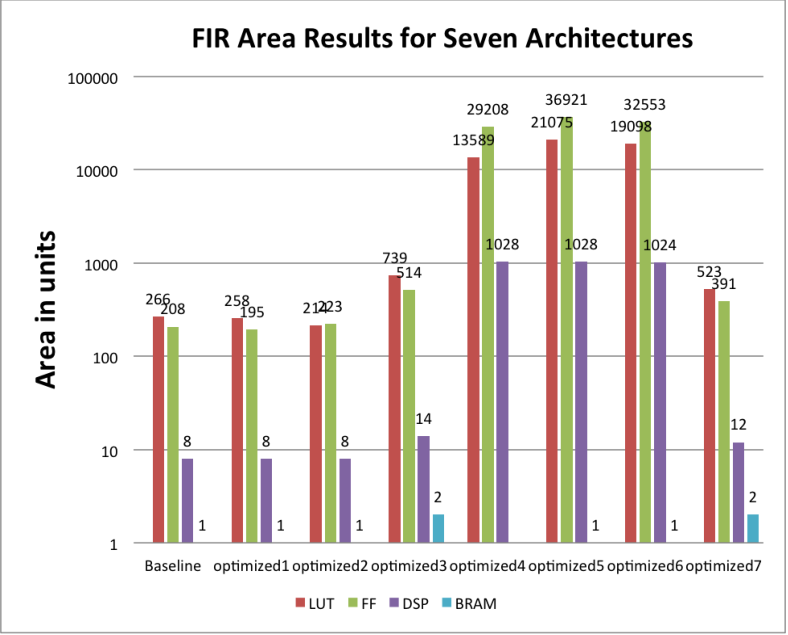
\includegraphics[width=5in]{images/fir_area_results}
\caption{The resource usage of eight different FIR architectures.}\label{fig:fir_area_results}
\end{figure}

\begin{figure}
\centering
%\includesvg{images/matrix_vector_sequential}
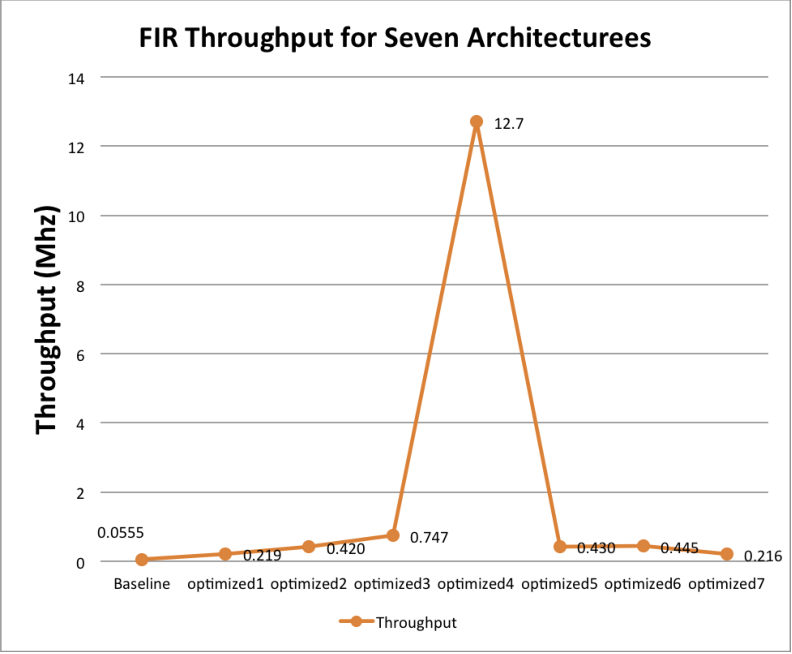
\includegraphics[width=5in]{images/fir_performance_results}
\caption{The throughput in terms of number of FIR outputs/second of eight different FIR architectures.}\label{fig:fir_performance_results}
\end{figure}

We calculated the throughput of the architectures in terms of number of FIR outputs per second. This requires that we calculate the total time that one call to the \texttt{fir()} function. The throughput is reported in Hz using the formula from Equation 2. We use the ``Estimated Clock Period (ns)'' from HLS report instead of the specified clock period. 

The throughput in Hertz can be calculated as:
\begin{equation}
Throughput (Hz) = \frac{1}{Clock\_Period (s) \cdot Num\_Clock \_Cycles}
\end{equation}                           	
The throughput in MHz can be calculated as:
\begin{align*}
Throughput (Mhz) = \frac{1}{Clock\_Period (s) \cdot Num\_Clock\_Cycles} \cdot \frac{1}{10^6} \\
  		                        = \frac{1000}{Clock\_Period (ns) \cdot Num\_Clock\_Cycles}                    
\end{align*}

You should always present your results using units (Hz, KHz, MHz, etc.) that make ``sense''. For example, you should not do 10000 Hz rather 10 KHz, and 200 KHz instead of .2 MHz.


\note{Remove the following two sections?}
\section{Submission Procedure}

You should submit a report that must include your results for the demo and each of the architecture that you generated for FIR128. For the FIR128, this report should plot the results,  e.g., resource utilization in terms of BRAMs, DSP48, FFs, LUTs, etc., and performance in terms of number of throughput (number of FIR operations/second), clock cycles, clock frequency (which is fixed to 10 ns). Your report should describe each of the architectures that you generated. You should discuss the exact optimization and its resulting architecture. Figures describing the architectures are highly encouraged.

You must also submit your code (and only your code, not other files). Your code should have everything in it so that we can synthesize it directly. This means that you should use pragmas in your code, and not use the GUI to insert optimization directives. Or you can insert the optimizations into your TCL script. We must be able to have all of the knowledge available to easily synthesize any and all of your designs.

The folder should be zipped with a similar file structure as below:
\texttt{FIR\_lab\_LASTNAME1\_LASTNAME2.zip}, where \texttt{LASTNAME2} is included if you are submitting a joint report with another person.

Contents:
\begin{itemize}
\item \texttt{report.pdf}
\item \texttt{demo\_picture}: A screenshot or pdf version of your plot graph from the demo.
\item Folder \texttt{baseline}: original unmodified \texttt{fir.cpp}.
\item Folder \texttt{optimized1} first optimization with \texttt{fir.cpp}.
\item Folder \texttt{optimized2}: second optimized design with \texttt{fir.cpp}
\item \dots
\item Folder \texttt{optimizedN}: nth optimized design with \texttt{fir.cpp}.
\end{itemize}
Each folder also must contain \texttt{script.tcl} file that can be used to create the project

\section{Grading Rubric}
The working demo of your code on the Zedboard will account for 60\% of your grade. You can document this in your report with a screenshot as well as some discussion as to any difficulties that you had during this implementation. Of course, we reserve the right to have you demo this for us in person. The remaining 40\% requires that you generate at least one architecture that uses each of the five listed optimizations (Variable Bitwidths, Removing Conditional Statements, Pipelining, Loop Fission, Memory Partitioning). 

The report should be well written and presented. Additional points (up to 20) will be subtracted for poor reports. Examples of issues include any spelling errors, multiple/egregious grammar, poor presentation of results, lack of written comparison of the results, etc. I expect there to be insights into the different architectures. Simply stating the optimizations that you did and presenting the results is not sufficient. You should attempt to answer questions as to why did this optimization produce better results. Why is one architecture better than the other? What sort of architecture is being generated? Etc. This will help you for future assignments so it is worthwhile spending time understanding the tools now.
